\section{Week 3}
\textbf{Key concepts of Root Locus Plot}
\begin{itemize}
    \item RL plots the coordinates of closed loop poles, $s$, given different $K$ values using CE: $1+K\cdot G(s) = 0$.
    \item RL starts ($K=0$) at open-loop poles, and ends ($K\to \infty$) at either open-loop zeros or asymptotes. 
    \item Adding open-loop poles makes the closed-loop system \textbf{less stable}.
    \item Adding open-loop zeros makes the closed-loop system \textbf{more stable}. 
\end{itemize}

\textbf{Given s-value, how to find K-value?}
\begin{itemize}
    \item Magnitude Condition \\
    \begin{equation*}
        \frac{|s+a_0|\times |s+a_1| \times \ldots |s+a_m|}{|s+b_0|\times |s+b_1| \times \ldots |s+b_m|} = \left|-\frac{1}{K}\right|
    \end{equation*}
    \item Angle Condition ($\theta$ away from x-axis) \\
    \begin{equation*}
        \sum_{i=1}^{m} \phase{(s+a_i)} - \sum_{j=1}^{n}\phase{(s+b_j)} = \phase{-\frac{1}{K}} = -180^{\circ} \; (\text{if $K>0$})
    \end{equation*}
\end{itemize}

\textbf{Root Locus Drawing Rules}
\begin{figure}[H]
    \centering
    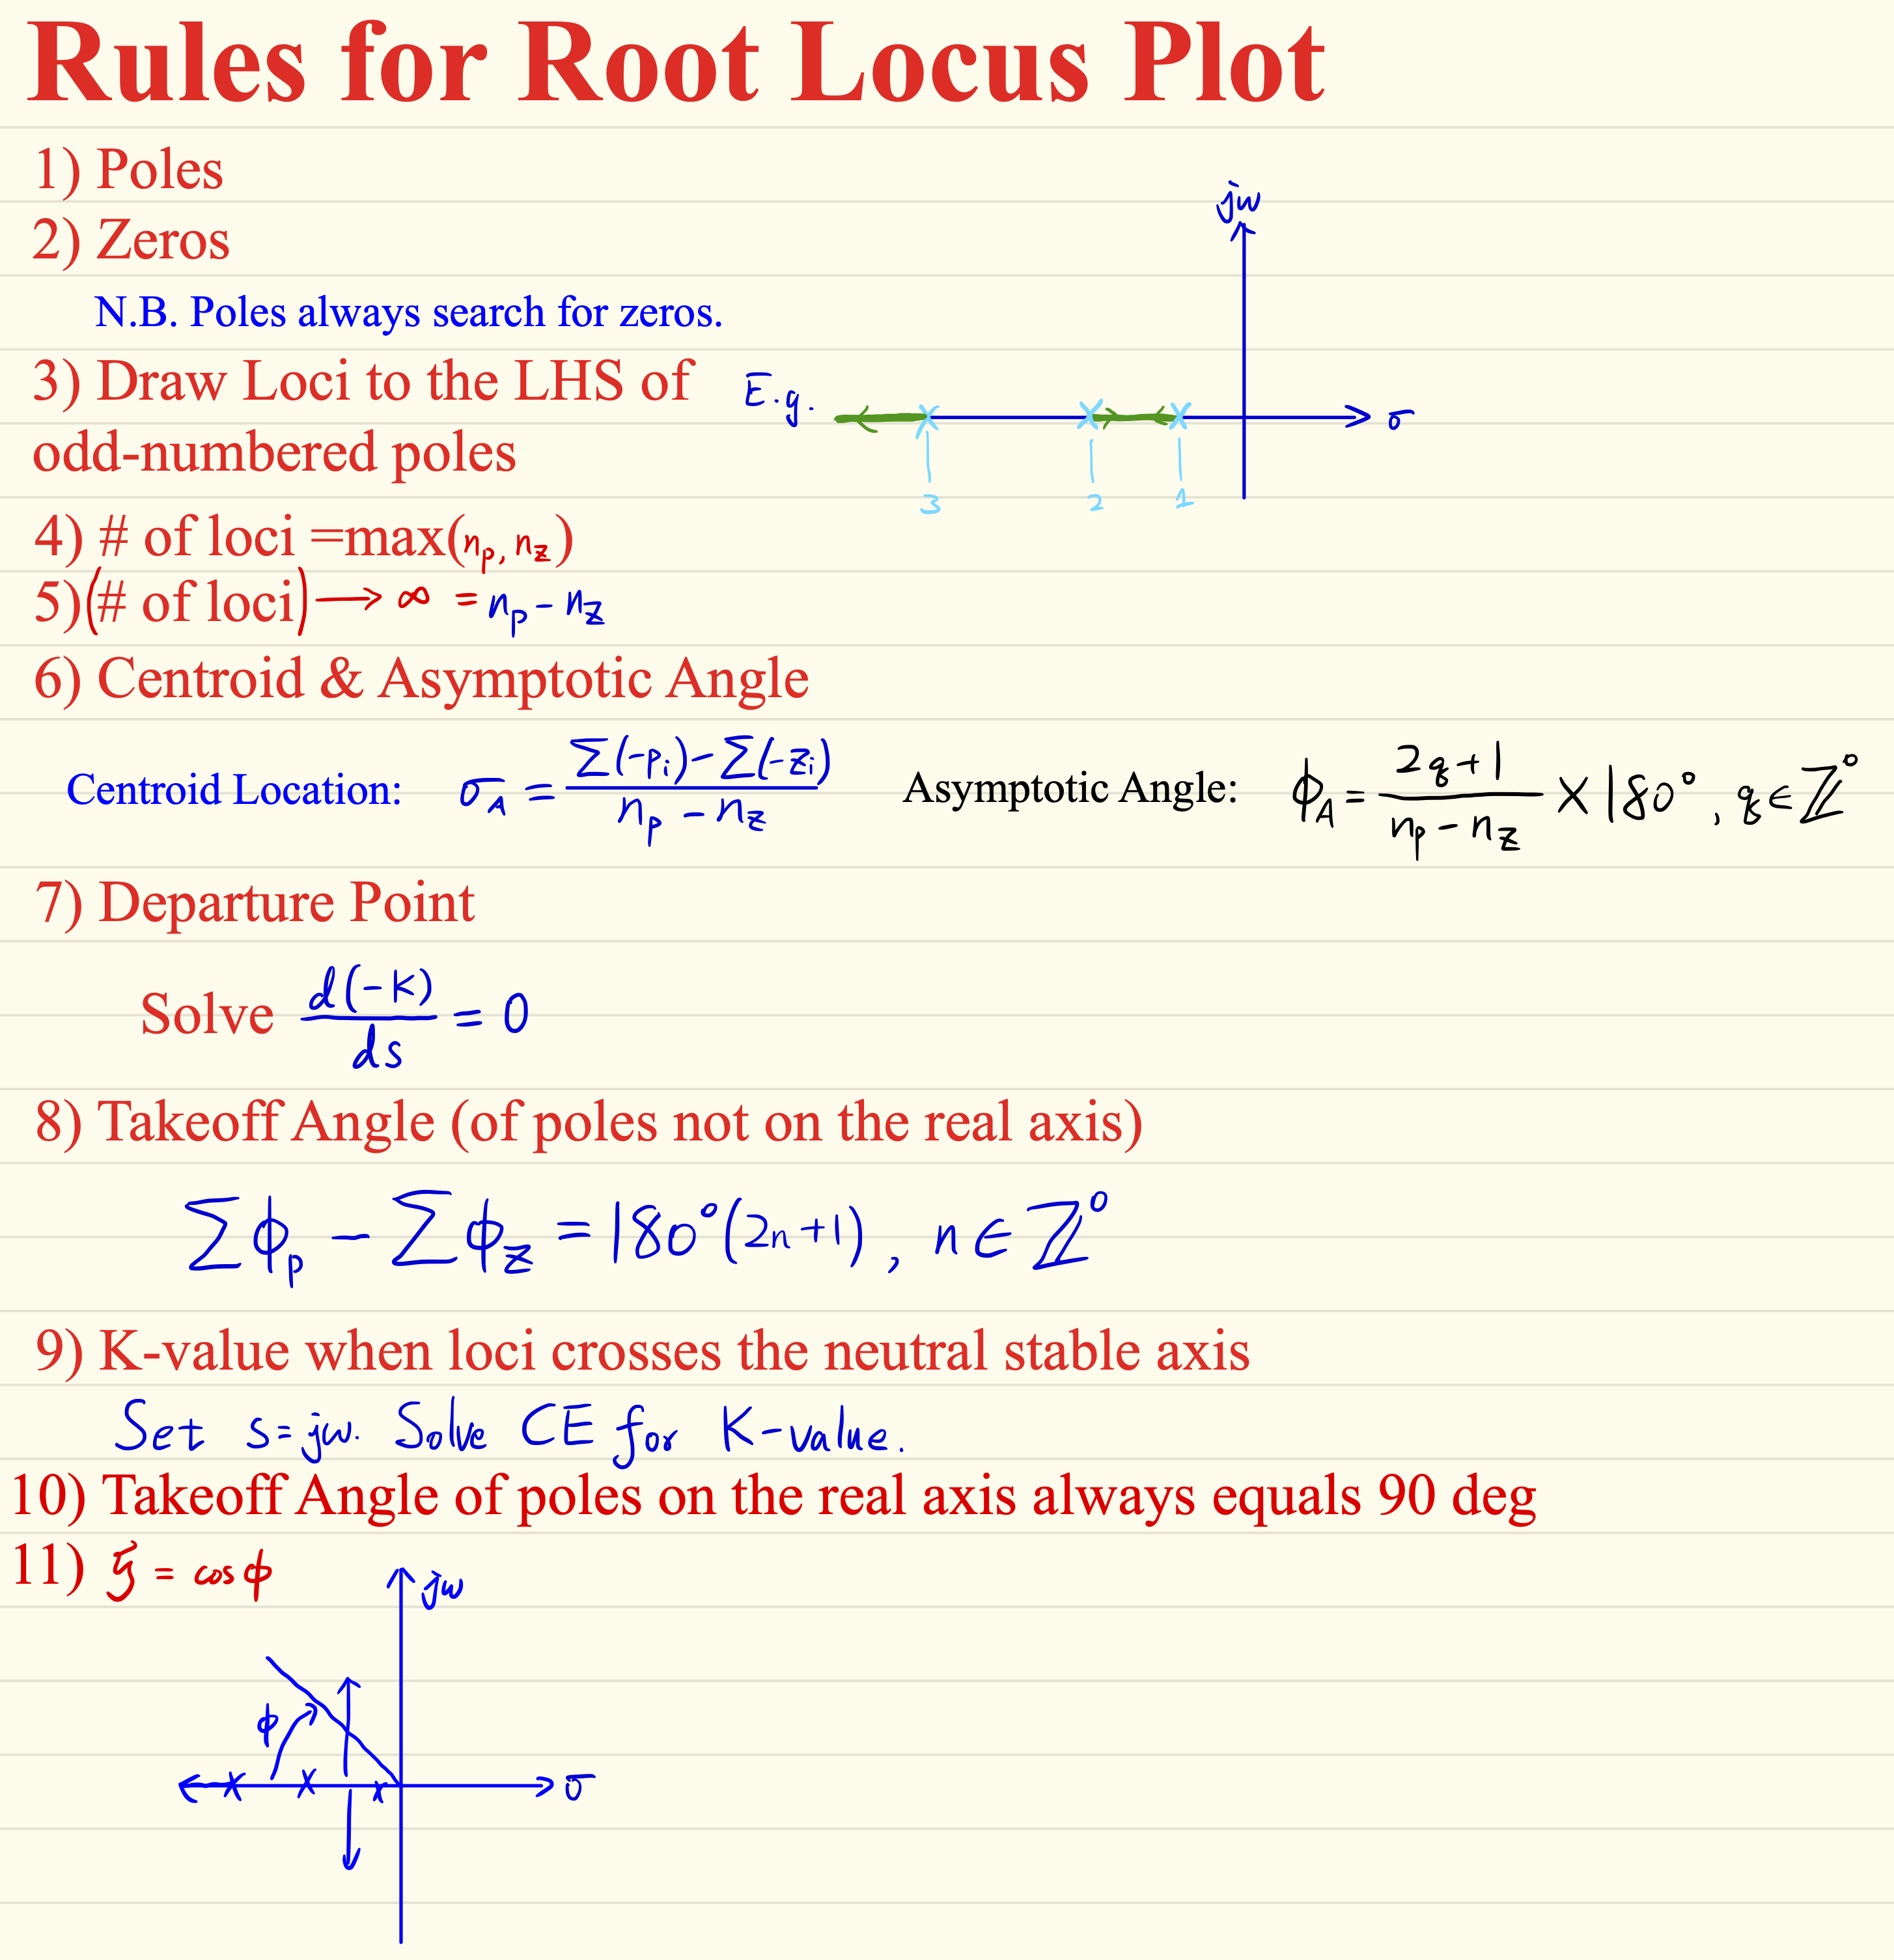
\includegraphics[width=0.5\textwidth]{images/root_locus_rules.png}
\end{figure}